\documentclass[11pt]{article}

\usepackage{amsmath}
\usepackage{amssymb}
\usepackage{graphicx}
\usepackage{caption}
\usepackage{subcaption}

\topmargin -.5in
\textheight 9in
\oddsidemargin -.25in
\evensidemargin -.25in
\textwidth 7in

\newcommand{\code}[1]{\texttt{#1}}

\begin{document}

\author{Gu, Qiao}
\title{16-720B Homework 4 Write-up}
\maketitle

\medskip

\subsection*{Q1.1}

The given translation is applied to all $x_j$ for $j\in \mathbb{R}$. Then for each $x_ii$

\begin{align}
  softmax(x_i+c) = \frac{e^{x_i+c}}{\sum_j e^{x_j+c}} = \frac{e^{x_i}e^c}{\sum_j e^{x_j}e^c}
  = \frac{e^{x_i}e^c}{(\sum_j e^{x_j})e^c} = \frac{e^{x_i}}{\sum_j e^{x_j}} = softmax(x_i).
\end{align}

This shows that softmax is invariant to translation.

When $c=-\max x_i$, all $x_i+c <0$ and $e^{x_i+c} \in (0,1)$, and the difference between $e^{x_I}$ is relatively small. And when $c=0$, $e^{x_i}$ can be exponentially large and may cause numerical instability.

\newpage

\subsection*{Q1.2}

\begin{itemize}
  \item Each element of softmax $softmax(x_i)$ is in range $(0,1)$, and the sum over all elements is $\sum_j softmax(x_j) = 1$.
  \item Probability.
  \item $s_i=e^{x_i}$ is to map each $x_i$ to its probability weight. $S=\sum s_i$ is find the sum of the weights. $softmax(x_I) = \frac{1}{S} x_i$ is to normalize each weight by all weights to get probability.
\end{itemize}

\newpage

\subsection*{Q1.3}

\newcommand{\bx} {\mathbf{x}}
\newcommand{\by} {\mathbf{y}}
\newcommand{\bW} {\mathbf{W}}
\newcommand{\bb} {\mathbf{b}}

Each layer of a neural network can be written mathmatically as $f_i(\bx)=\bW_i\bx+\bb$, and thus is we concatenate $n$ layers together without non-linear layers, we get the output as

\begin{align}
  \by &= f_n(f_{n-1}(\cdots f_1(\bx) \cdots)) \\
  &= \bW_n (\bW_{n-1} (\cdots(\bW_1\bx+\bb_1)\cdots) +\bb_{n-1}) + \bb_n \\
  &= \bW_n \bW_{n-1}\cdots \bW_1 \bx + \bW_n \bW_{n-1}\cdots \bW_2 \bb_1 + \bW_n \bW_{n-1}\cdots \bW_3 \bb_2 + \cdots + \bW_n\bb_{n-1} + \bb_n\\
  &= \bW\bx+b,
\end{align}

where $\bW = \bW_n \bW_{n-1}\cdots \bW_1$ and $\bb = \bW_n \bW_{n-1}\cdots \bW_2 \bb_1 + \bW_n \bW_{n-1}\cdots \bW_3 \bb_2 + \cdots + \bW_n\bb_{n-1} + \bb_n$. This can be regarded as a single linear layer, and the whole network is equivalent to linear regression.

\newpage

\subsection*{Q1.4}

\begin{align}
  \frac{d\sigma(x)}{dx} &= \frac{d}{dx}\frac{1}{1+e^{-x}} \\
  &= (-1)\frac{1}{(1+e^{-x})^2} \frac{d}{dx} (1+e^{-x}) \\
  &= (-1)\frac{1}{(1+e^{-x})^2} (-e^{-x}) \\
  &= \frac{1+e^{-x}-1}{(1+e^{-x})^2} \\
  &- \frac{1}{1+e^{-x}} - \frac{1}{(1+e^{-x})^2} \\
  &= \frac{1}{1+e^{-x}} (1-\frac{1}{1+e^{-x}}) \\
  &= \sigma(x) (1-\sigma(x))
\end{align}

\newpage
\subsection*{Q1.5}

\newcommand{\bdelta} {\mathbf{\delta}}

The loss function is unknown and therefore we assume $\frac{\partial J}{\partial y_i} = \delta_i$. Therefore

\begin{align}
  \frac{\partial J}{\partial W_{ij}} &= \frac{\partial J}{\partial y_i} \frac{\partial y_i}{\partial W_{ij}} = \delta_i x_j \\
  \frac{\partial J}{\partial x_j} &= \sum_{i=0}^k \frac{\partial J}{\partial y_i}\frac{\partial y_i}{\partial x_j} = \delta_i \sum_{i=0}^k W_{ij} \\
  \frac{\partial J}{\partial b_i} &= \frac{\partial J}{\partial y_i} \frac{\partial y_i}{\partial b_i} = \delta_i
\end{align}

And then we can further rewrite it to matrix form

\begin{align}
  \frac{\partial J}{\partial\bW} &= \bdelta \bx^T \\
  \frac{\partial J}{\partial\bx} &= \bW^T \bdelta \\
  \frac{\partial J}{\partial\bb} &= \bdelta
\end{align}

\newpage

\subsection*{Q1.6}

\begin{enumerate}
    \item As shown in Figure.~\ref{fig:q1.6.1}, when the input to the sigmoid $x$ is far away from zero, the magnitude of the gradient becomes very close to zero and thus the gradient from higher layers are scaled by a very small number, even "vanishing". Therefore, when we update the network weights, the changes will be very small.
    \item The output range of sigmoid function is $(0,1)$ and the output range of $tanh(x)$ is $(-1,1)$. If our input data are centered at 0, the output given by $\tanh$ are also centered at 0, which will make the input to different layers consistent.
    \item From Figure.~\ref{fig:q1.6.1}, we can see that $\tanh(x)$ has a stronger gradient (larger magnitude) than $\sigma(x)$ does.
    \item $\tanh(x)=2\sigma(2x)-1$ as
    \begin{align}
    \begin{split}
        \sigma(x) = \frac{1}{1+e^{-x}}
        &\Rightarrow \sigma(2x) = \frac{1}{1+e^{-2x}}
        \Rightarrow 2\sigma(2x) = \frac{2}{1+e^{-2x}} \\
        &\Rightarrow 2\sigma(2x)-1 = \frac{2-1-e^{-2x}}{1+e^{-2x}} = \frac{1-e^{-2x}}{1+e^{-2x}} = \tanh(x)
    \end{split}
    \end{align}
\end{enumerate}

\begin{figure}[h!]
    \centering
    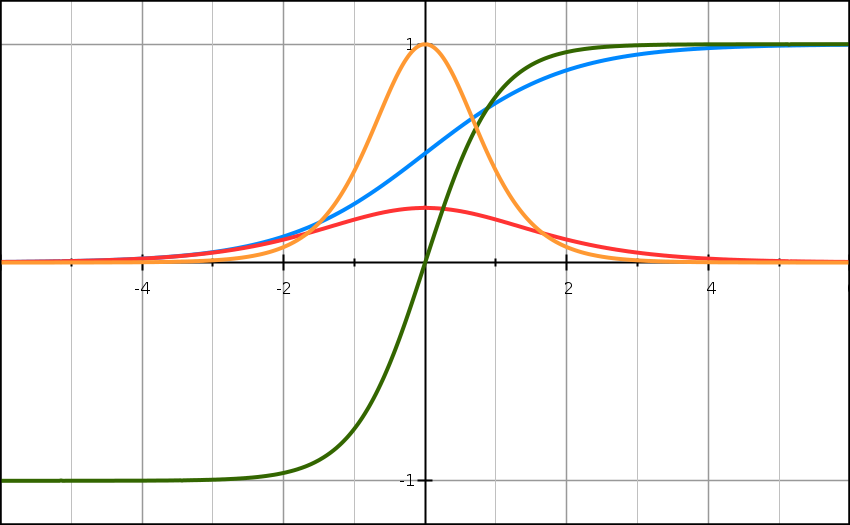
\includegraphics[width=.6\linewidth]{../results/q1_6_1.png}
    \caption{The plot of sigmoid function $\sigma(x)$ (in blue), its gradient $(1-\sigma(x))\sigma(x)$ (in red), the $\tanh(x)$ function (in green) and its gradient $1-\tanh^2(x)$ (in orange). }
    \label{fig:q1.6.1}
\end{figure}

\newpage

\subsection*{Q2.1.1}

If the weights and biases of every layer are initialized with zeros, the outpuut layer pre-activation values will be zeros regardless the input data and the post-activation values will be a uniform probability distribution.
In this case, there will still be gradients in the network due to the softmax loss, but they will be very small. Therefore the update of the network is very slow, the training process may terminate without convergence or the network may be stuck at local optima.
% Therefore The gradients of the network therefore will be zeros during training and the network weights will remain zeros after training.

\newpage

\subsection*{Q2.1.3}

Because if we initialize all the weights with the same number, some of them will have the same effect on the output values, and the gradients on them will be the same during backpropagation. Therefore, they will move together and hard to converge during training.

Because in one layer of neural net $\by=\bW\bx+\bb$, the variance of the output $\by$ depends on both the variance of input $\bx$ and variance of elements of the weight $\bW$. This is also true during the backpropagation of gradients. Therefore we scale the weight variance down by the layer size, To make the output variance of each layer equal to the input variance.

\newpage

\subsection*{Q3.1.2}

The progression of the loss and accuracy during the training process is shown in Figure.~\ref{fig:q3.1.2}. Here the best learning rate I found is $2\times10^{-3}$.

Learning rates affect training process in the sense that the best learning rate gives the best convergence. Overly high or overly low learning rates will both slow down the convergence or make the training not able to converge to local optima.

Additionally, we can notice that large learning rates may cause the learning process to overshoot, which causes accuracy and loss to fluctuate during the training process.

The final test accuracy of the best network is $78\%$.

\begin{figure}[h!]
    \begin{subfigure}{.325\textwidth}
      \centering
      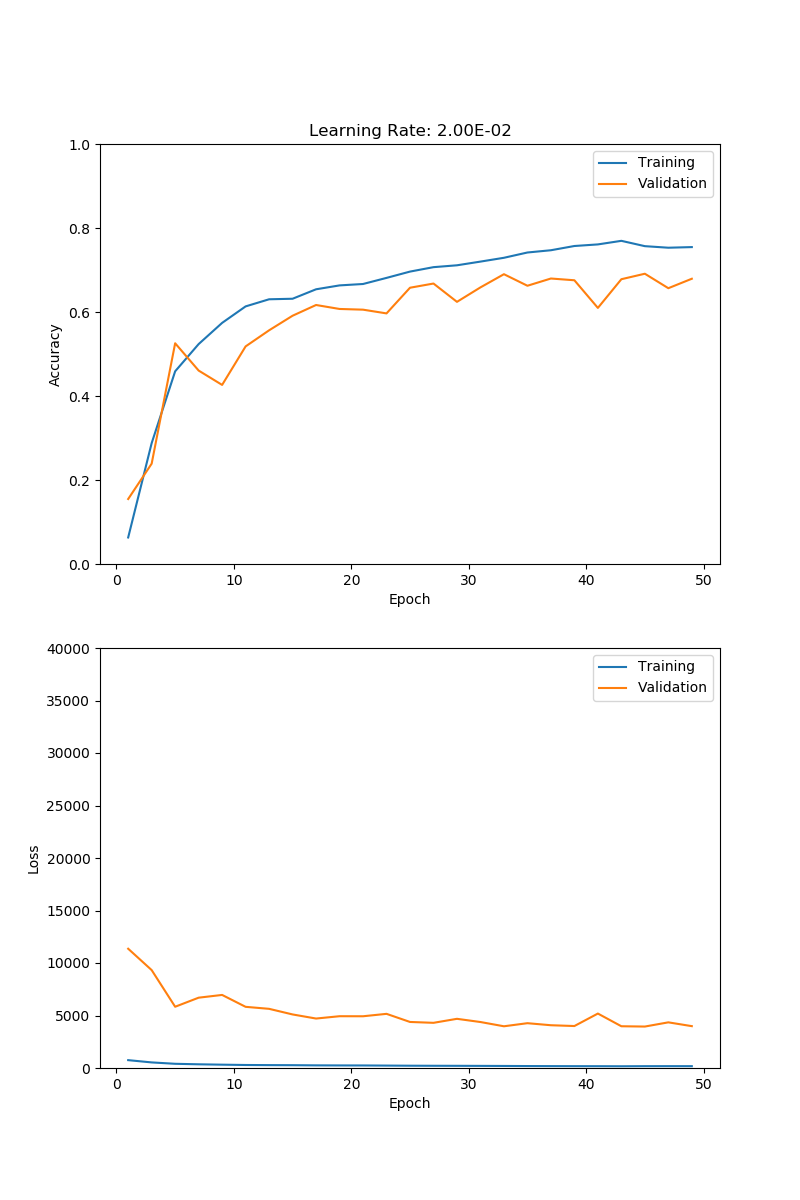
\includegraphics[width=.95\linewidth]{../results/q3_1_2_2E-02.png}
      \caption{Learning rate = $2\times10^{-2}$}
    \end{subfigure}
    \begin{subfigure}{.325\textwidth}
      \centering
      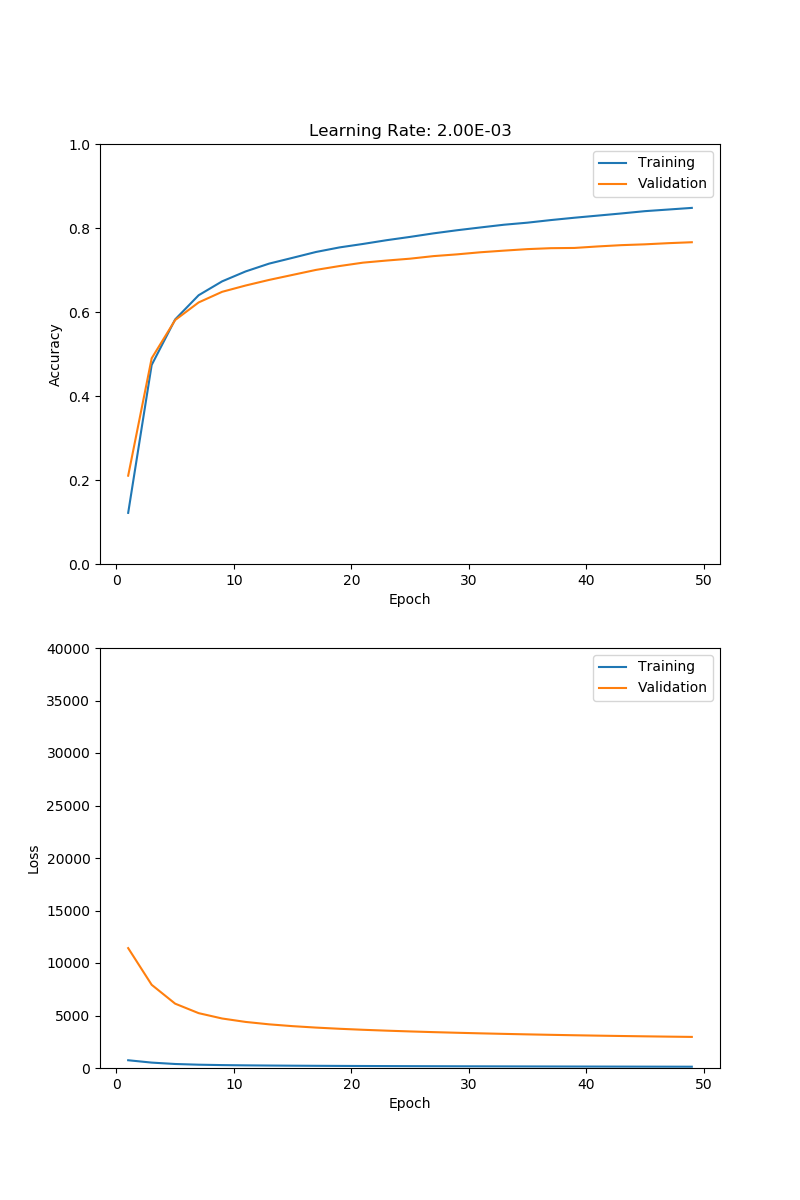
\includegraphics[width=.95\linewidth]{../results/q3_1_2_2E-03.png}
      \caption{Learning rate = $2\times10^{-3}$}
    \end{subfigure}
    \begin{subfigure}{.325\textwidth}
      \centering
      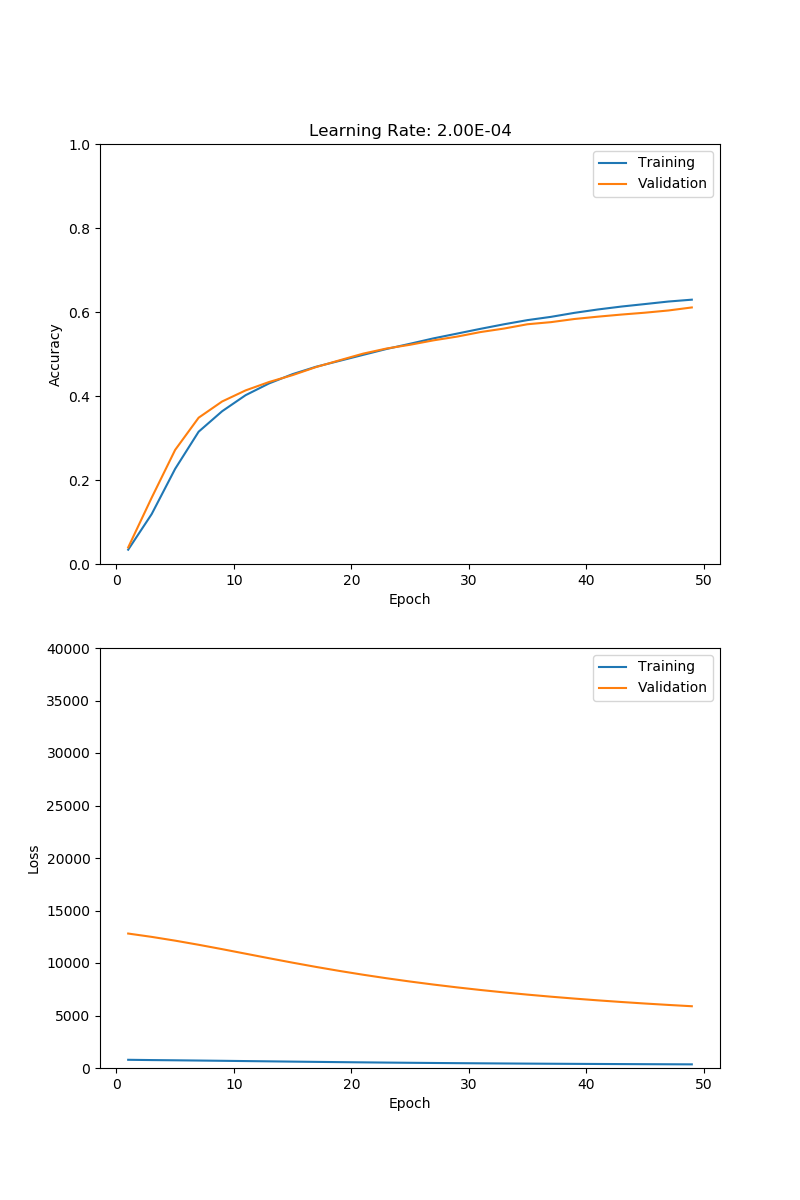
\includegraphics[width=.95\linewidth]{../results/q3_1_2_2E-04.png}
      \caption{Learning rate = $2\times10^{-4}$}
    \end{subfigure}\hfill
    \caption{Training progress on loss and accuracy using different learning rates. }
    \label{fig:q3.1.2}
\end{figure}

\newpage

\subsection*{Q3.1.3}

The weights of the first layer of the network is visualized in Figure.~\ref{fig:q3.1.3}. As we can observe, the weights after training is more structured and some of them resemble stroke curves of different digits and characters, and thus when we apply these weights, the input image that have similar strokes will have higher activation.

And before training, the visualized weights are just random noise and no structures or patterns can be observed.

\begin{figure}[h!]
    \begin{subfigure}{.495\textwidth}
      \centering
      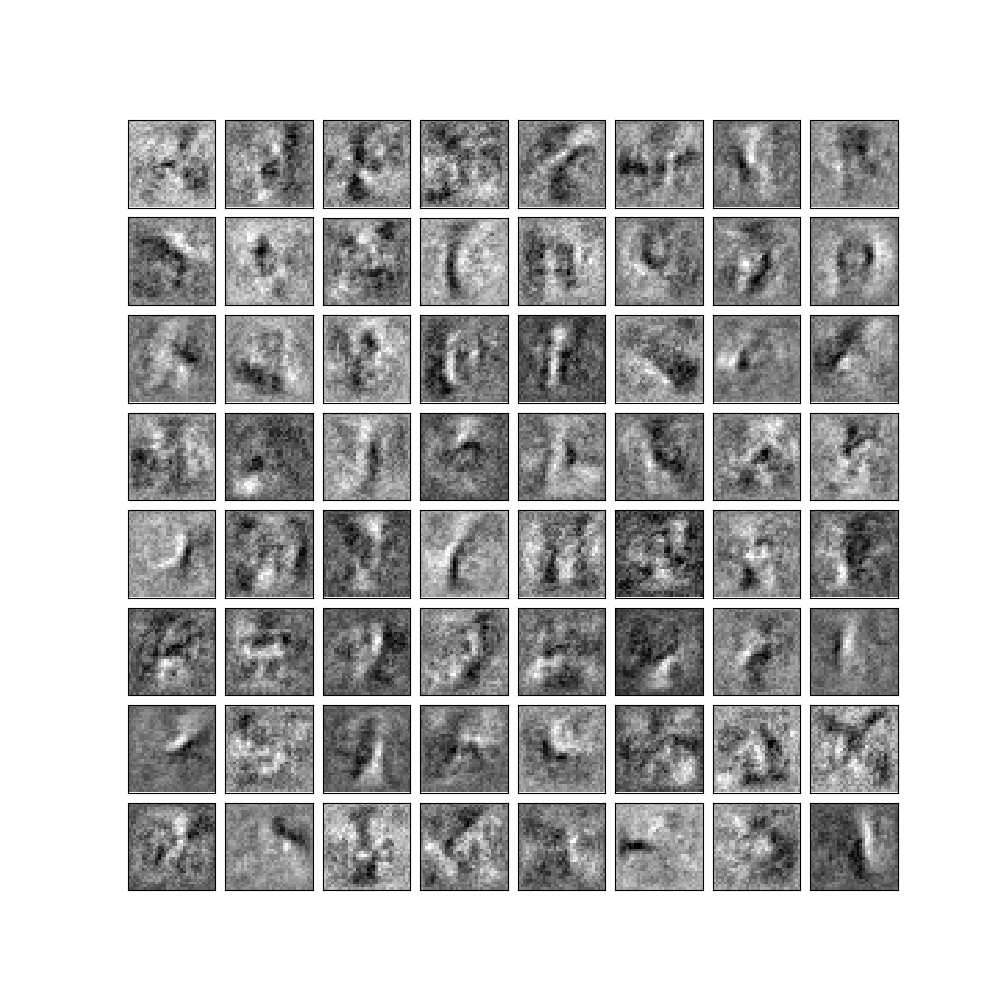
\includegraphics[width=.95\linewidth]{../results/q3_1_3a.png}
      \caption{After training}
    \end{subfigure}
    \begin{subfigure}{.495\textwidth}
      \centering
      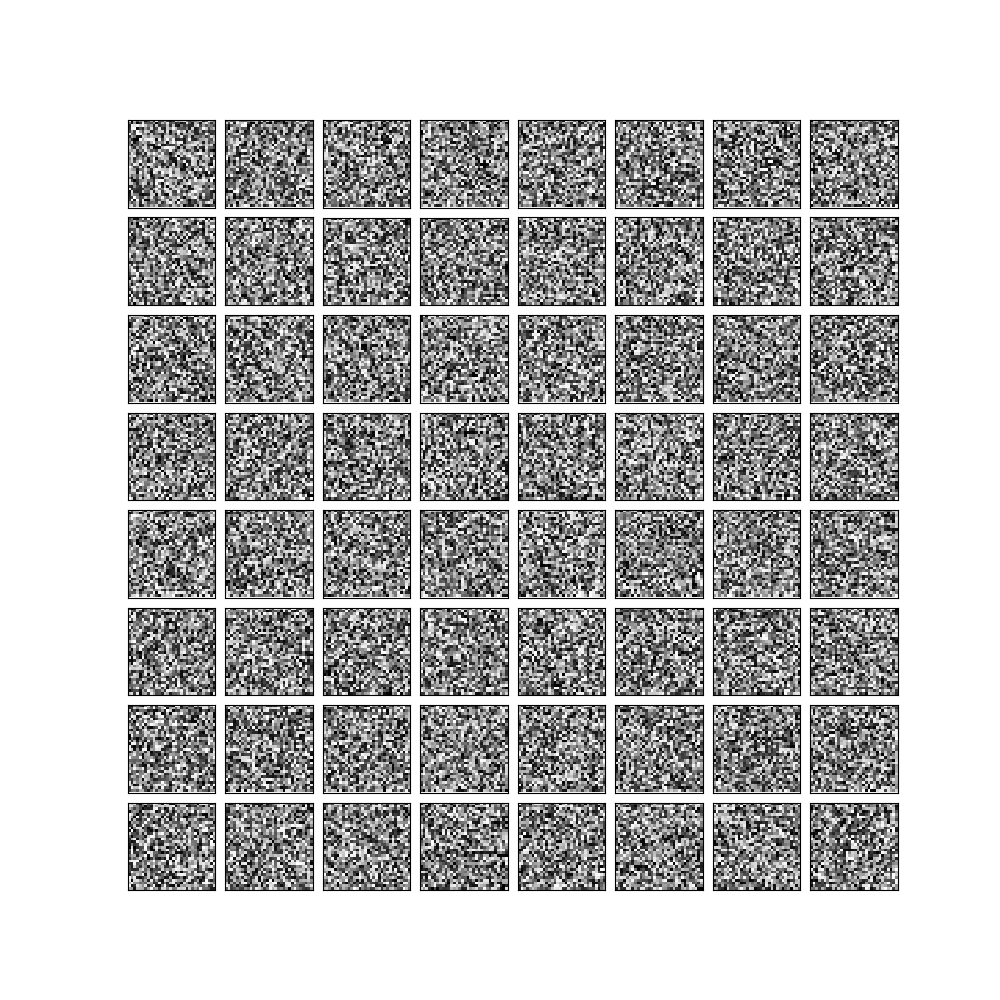
\includegraphics[width=.95\linewidth]{../results/q3_1_3b.png}
      \caption{Before training}
    \end{subfigure}\hfill
    \caption{Visualization of weights before and after training. }
    \label{fig:q3.1.3}
\end{figure}

\newpage

\subsection*{Q3.1.4}

The confusion matrix of the best model on the validation dataset is shown in Figure.~\ref{fig:q3.1.4}. As shown by some entries with high values in the matrix, the network is likely mix the digit ``0'' with the character `'O'', the character ``S'' with the digit ``5'', and digit ``1'' with character ``I''. These results are quite reasonable as these pairs have very similar shape and even some human can get confused by them.

\begin{figure}[h!]
    \centering
    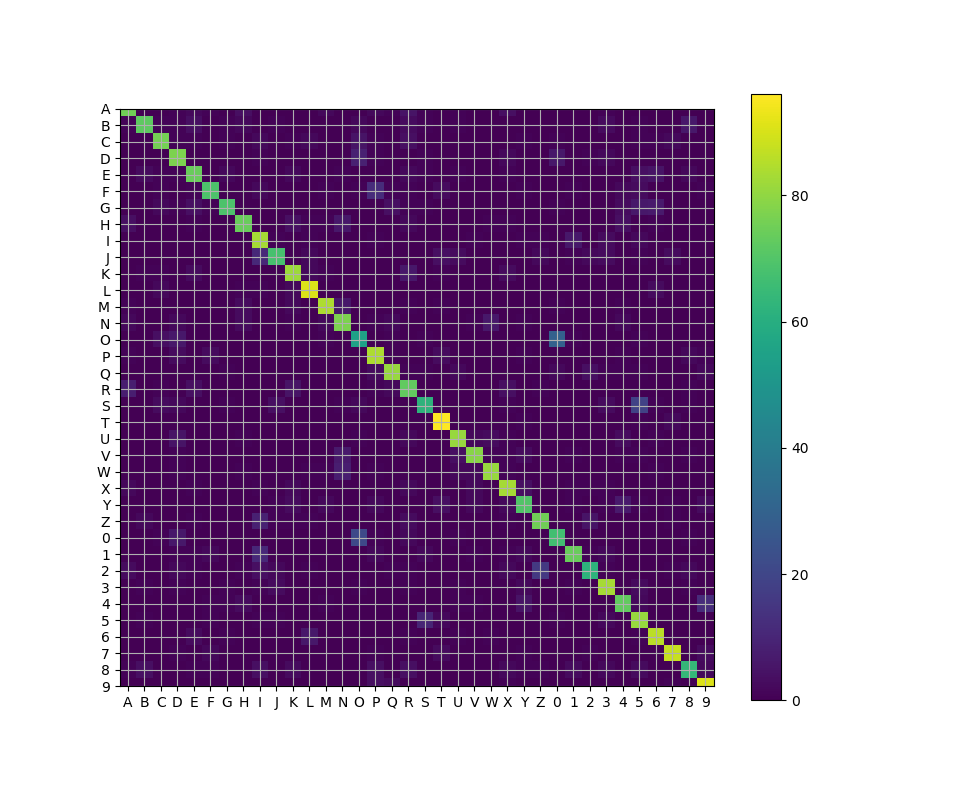
\includegraphics[width=.8\linewidth]{../results/q3_1_4.png}
    \caption{The confusion matrix of the best model on the validation dataset ($N=3600$). }
    \label{fig:q3.1.4}
\end{figure}

\newpage

\subsection*{Q4.1}

The first assumption made is that each character is connected within itself and well separate from others, which means the method could fail if a character is splitted by background pixels or is connected to others by foreground pixels. Some examples where the method could fail are shown in Figure.~\ref{fig:q4.1} (a).

The second assumption is that all character are written in the upright form (no large rotation is applied), each line of text is written horizontallly and text is written line by line. The method could fail if the text are written with large rotation, as shown in Figure.~\ref{fig:q4.1} (b).

\begin{figure}[h!]
    \begin{subfigure}{.495\textwidth}
      \centering
      
\includegraphics[width=.5\linewidth]{../results/q4_1a.png}
      \caption{The characters that are connected to each other (``ABC'') or divided into multiple parts (``D''). }
    \end{subfigure}
    \begin{subfigure}{.495\textwidth}
      \centering
      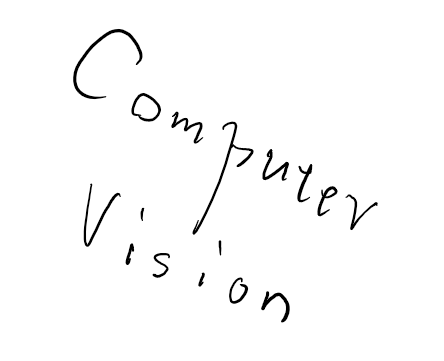
\includegraphics[width=.5\linewidth]{../results/q4_1b.png}
      \caption{The characters that are not written in horizontal and rotated. }
    \end{subfigure}\hfill
    \caption{Possible failure cases of the text extraction pipeline. }
    \label{fig:q4.1}
\end{figure}

\newpage

\subsection{Q4.3}

The character detection results are shown in Figure.~\ref{fig:q4.3}. Note that the bounding boxes are directly estimate from the connected pixels and thus they are not padded by now.

\begin{figure}[h!]
    \begin{subfigure}{.495\textwidth}
      \centering
      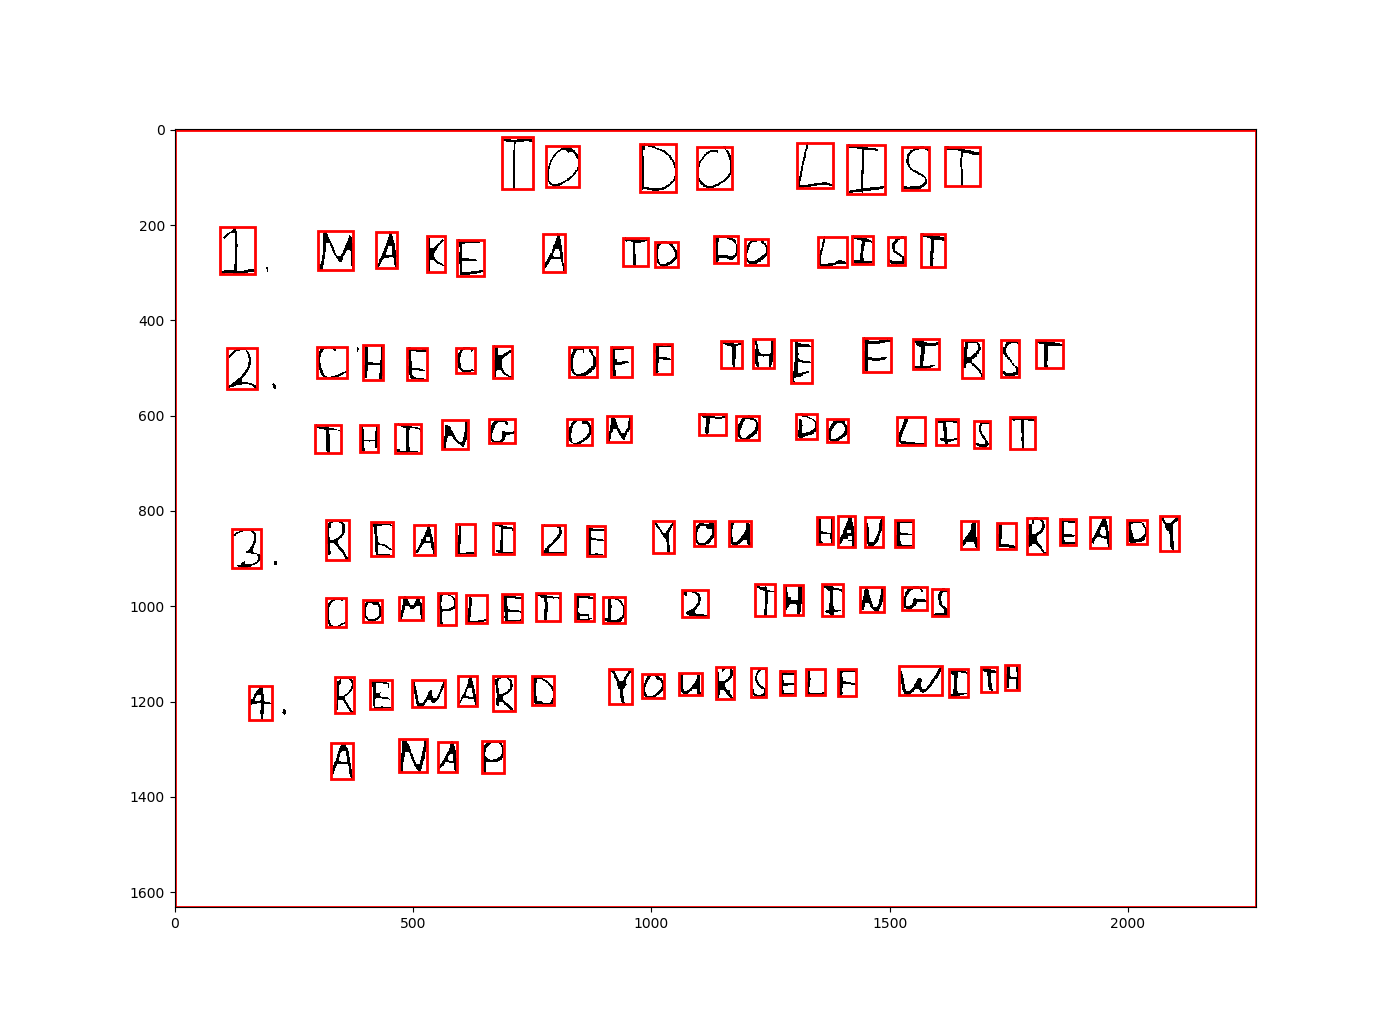
\includegraphics[width=.9\linewidth]{../results/q4_3_1.png}
      \caption{The detection result of the first image. }
    \end{subfigure}
    \begin{subfigure}{.495\textwidth}
      \centering
      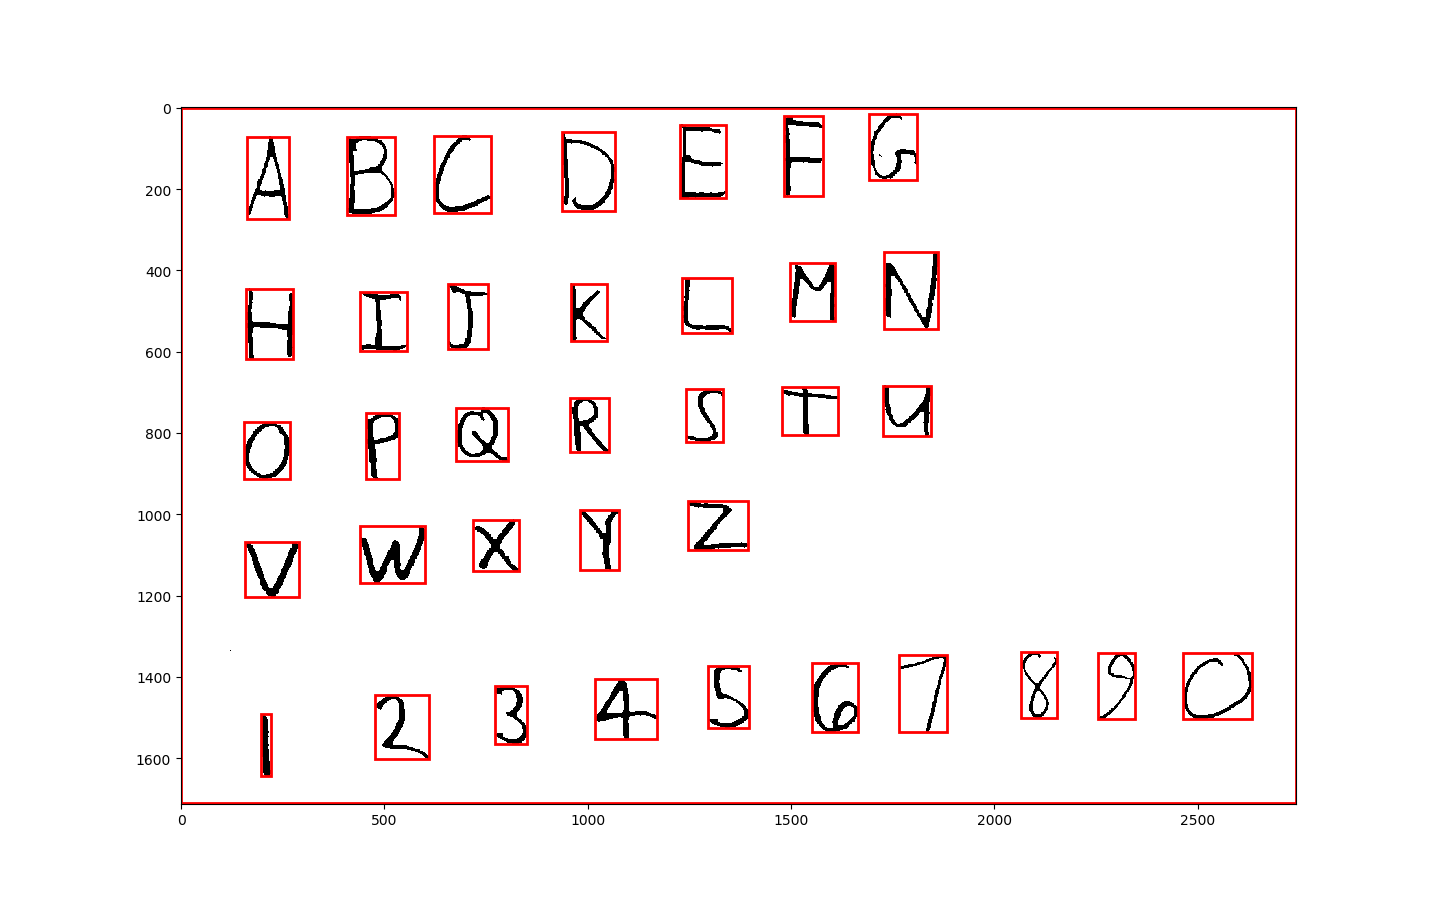
\includegraphics[width=.9\linewidth]{../results/q4_3_2.png}
      \caption{The detection result of the second image. }
    \end{subfigure}\hfill
    \begin{subfigure}{.495\textwidth}
      \centering
      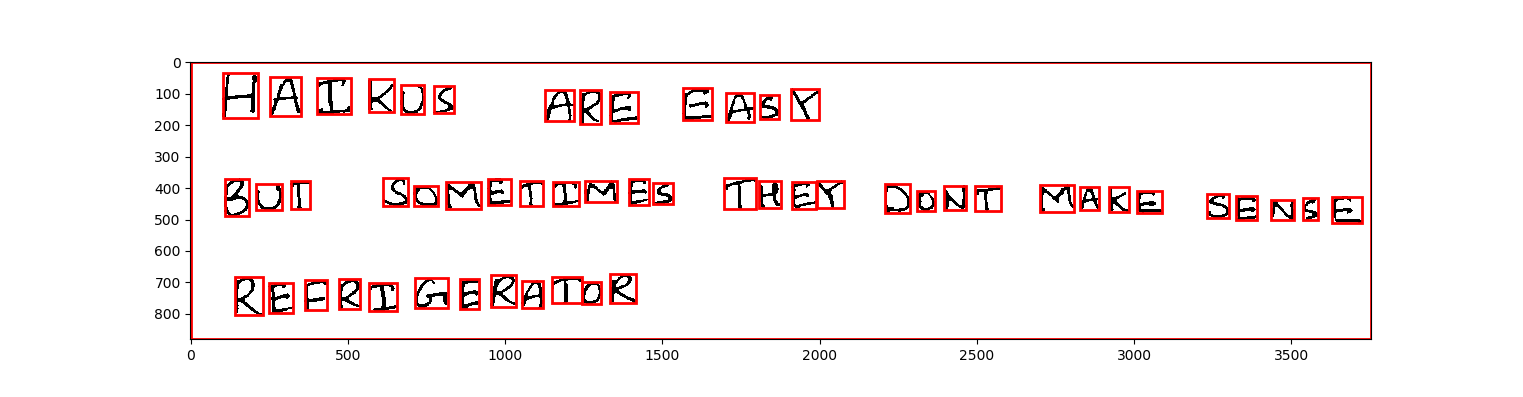
\includegraphics[width=.9\linewidth]{../results/q4_3_3.png}
      \caption{The detection result of the third image. }
    \end{subfigure}
    \begin{subfigure}{.495\textwidth}
      \centering
      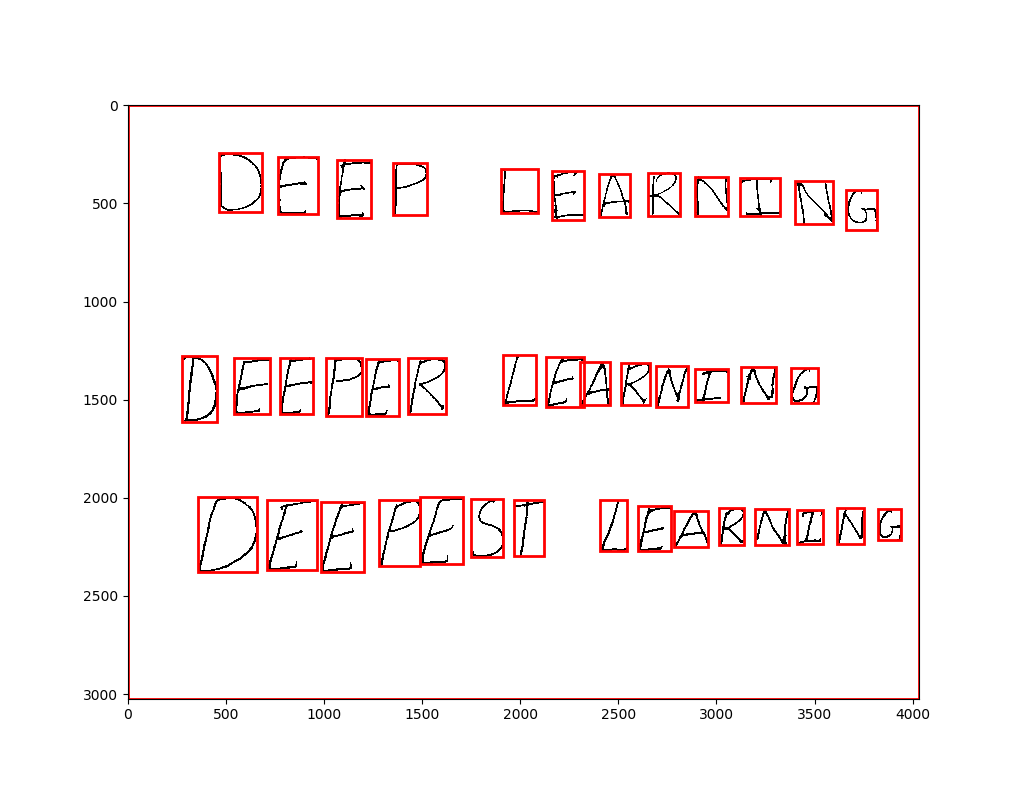
\includegraphics[width=.9\linewidth]{../results/q4_3_4.png}
      \caption{The detection result of the fourth image. }
    \end{subfigure}\hfill
    \caption{Detection results of characters in images in bounding boxes. }
    \label{fig:q4.3}
\end{figure}

\newpage
\subsection*{Q4.4}

The extracted texts are shown as follows:

\begin{verbatim}
T0D0LI5T
IMAKEAT0DOLIST
2CHFCK0FETHIFIRST
THING0NT0O0LIST
3RIALIZEY0UHAVEALR2ADT
C0MPL5T5D2THINGS
4XXWARDY0URSELFWITH
ANAP

XBCDEFG
HITKLMN
0PQRSTU
VWXYZ
1X3GS67X90

HAIKUSAREEASY
EUTSQMETIMESTREYD0NTMAK2SENQE
REFRIGERAT0R

DEEPLEARMING
CEEPTRLEARNING
5EEAE5TIEARNING
\end{verbatim}

\newpage

\subsection*{Q5.2}

The plotted training loss is shown in Figure.~\ref{fig:q5.2}.

As training process progresses, the training loss first drops quickly and then plateau at the low level.

\begin{figure}[h!]
    \centering
    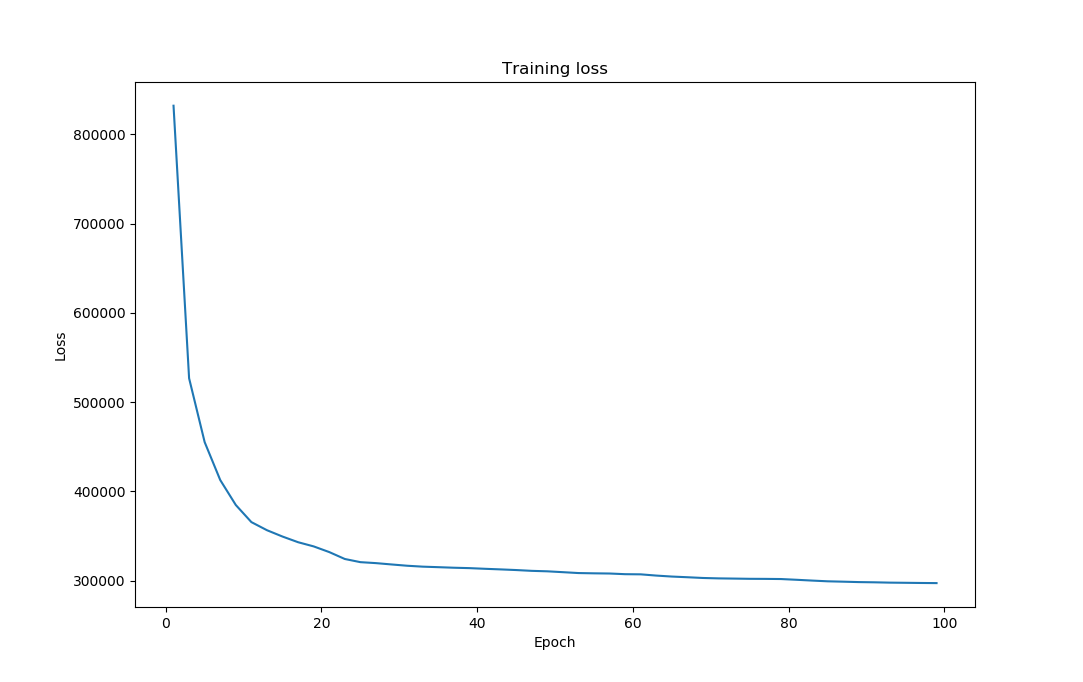
\includegraphics[width=.8\linewidth]{../results/q5_2.png}
    \caption{The training loss curve of the Autoencoder. }
    \label{fig:q5.2}
\end{figure}

\newpage

\subsection*{Q5.3.1}

The validation images and their reconstructions results are shown in Figure.~\ref{fig:q5.3.1}. As shown in the figure, the reconstructions results is more blur compared to the input images. Moreover, there is circle ``area of reconstruction'', and the contents within that circle can be better reconstructed than those outside (As shown by the first row of Figure.~\ref{fig:q5.3.1}). This is probably because the contents of training images are mostly centered in that circle.

\begin{figure}[h!]
    \centering
    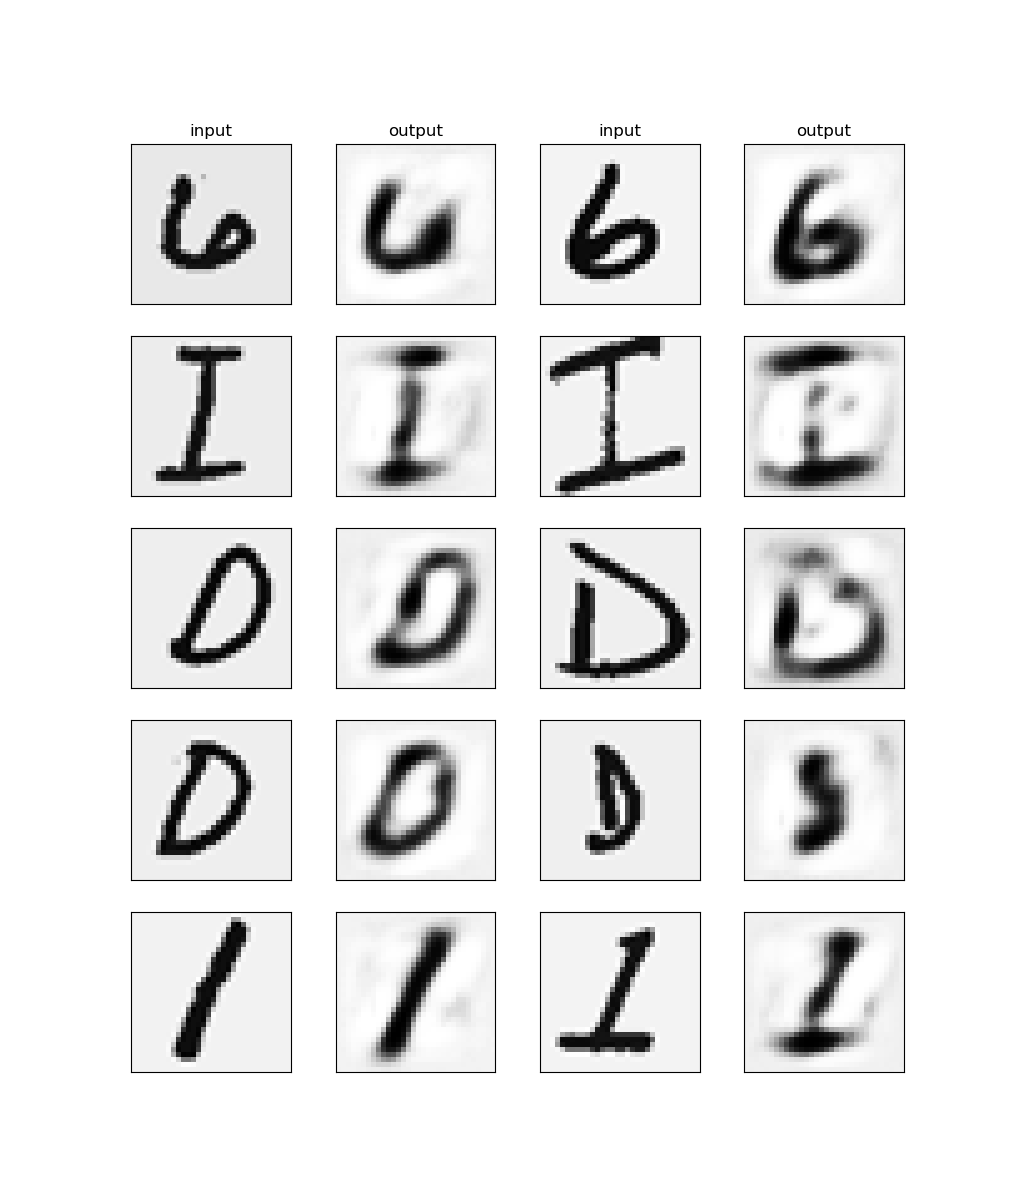
\includegraphics[width=.8\linewidth]{../results/q5_3_1.png}
    \caption{The validation images (input) and their reconstructions (output). }
    \label{fig:q5.3.1}
\end{figure}

\newpage

\subsection{Q5.3.2}

The average PSNR over the validation set is 16.084.

\end{document}
